\documentclass{article}

\usepackage{graphicx} % for images
\usepackage{amsmath} % for math
\usepackage{amssymb} % for \mathbb
\usepackage{siunitx} % for \SI, \num
\usepackage{hyperref} % for \url{}

% This stuff is for figures
\usepackage{float}
\DeclareGraphicsExtensions{.pdf, .png, .jpg}

% coloring of links for PDF format
\hypersetup{
    colorlinks=true,
    urlcolor=blue,
    linkcolor=black
}

% \c command redefinition (for monospaced font)
\renewcommand{\c}[1]{\texttt{#1}}
% \today command re-definition
%https://tex.stackexchange.com/questions/112932/today-month-as-text
\renewcommand{\today}{\ifnum\number\day<10 0\fi \number\day \space%
\ifcase \month \or January\or February\or March\or April\or May%
\or June\or July\or August\or September\or October\or November\or December\fi\space%
\number \year} 

\begin{document}

\noindent
Rodrigo Becerril Ferreyra\\
CECS 346 Section 03\\
Lab 4\\
\today

%\addcontentsline{toc}{section}{Introduction}
\section{Introduction}
The purpose of this lab was to set up and test an external
part called a proximity sensor. The proximity sensor is a
\SI{5}{\volt} system that changes its output signal to reflect
whether or not it detects an object in front of it. The
program used to test the sensor uses the on-board RGB LED
to display the state of the entire system: if the LED is green,
then the sensor does not sense anything; if the LED is blue,
then the sensor senses an object in front of it; a flashing
red LED represents a transition between the previous two states.
In addition, all inputs are treated for mechanical bounce.

\section{Hardware}
As previously stated, I am using an
infrared-radiation proximity sensor to drive the project.
Its \c{signal} output is connected to pin \c{B[0]}. To avoid
random movement and unpredictable triggering of the sensor,
it is taped to a cardboard box for stability.

To change the desired minimum range that the sensor detects
objects at, it is required to turn the potentiometer to
adjust its resistance. However, when I tried to turn it with a
screwdriver, the plastic wore out and I was unable to turn it.
I had to unsolder the potentiometer and re-solder in one of my
own. Even with this modification, I could not get the sensor
to detect anything farther away than approximately \SI{8}{cm}.

\section{Software}
Internally, the system uses three different interrupts:
one for Port B (where the sensor was connected), one for
Port F (where the two on-board buttons \c{SW1} and \c{SW2}
are connected), and one for the SysTick timer. The SysTick
timer is used to time the delays for the flashes for the
transition between the two main states. If the current state
of the LED is green, when the sensor detects
an object, the LED transitions from green to blue (green
$\rightarrow$ flashing red $\rightarrow$ blue). Pressing
\c{SW1} also achieves this, while pressing \c{SW2} has no effect.
Conversely,
if the current state
of the LED is blue, when the sensor stops detecting
an object, the LED transitions from blue to green (blue
$\rightarrow$ flashing red $\rightarrow$ green). Pressing
\c{SW2} also achieves this, while pressing \c{SW1} has no effect.

Debounce is implemented simply by waiting a certain amount of
time after an interrupt is triggered before handling the
interrupt. If the interrupt trigger condition is no longer
true, then the interrupt service routine is not executed.

\section{Media}
\begin{itemize}
\item A YouTube video of a demonstration of the system can be
found here: \url{https://youtu.be/Y_fqIKj0XAg}
\item The Figure %\ref{diagram:schematic}
is a schematic diagram of the system.
\begin{figure}[H]
    \centering
    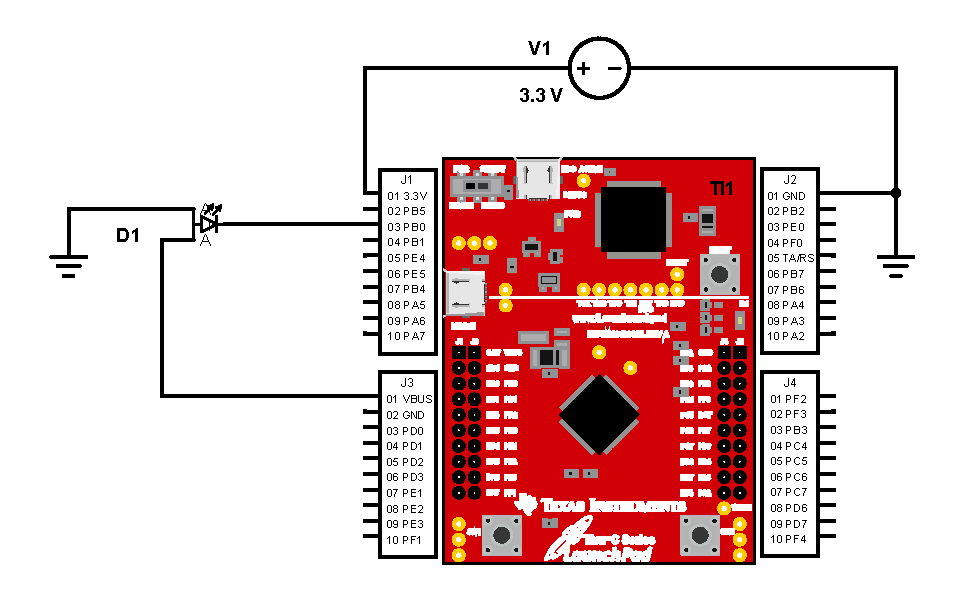
\includegraphics[width=\textwidth]{Images/schemeit-project}
    \caption{Schematic diagram of the system.}
    \label{diagram:schematic}
\end{figure}
\item The Figure \ref{image} is an image of the system.
\begin{figure}[H]
    \centering
    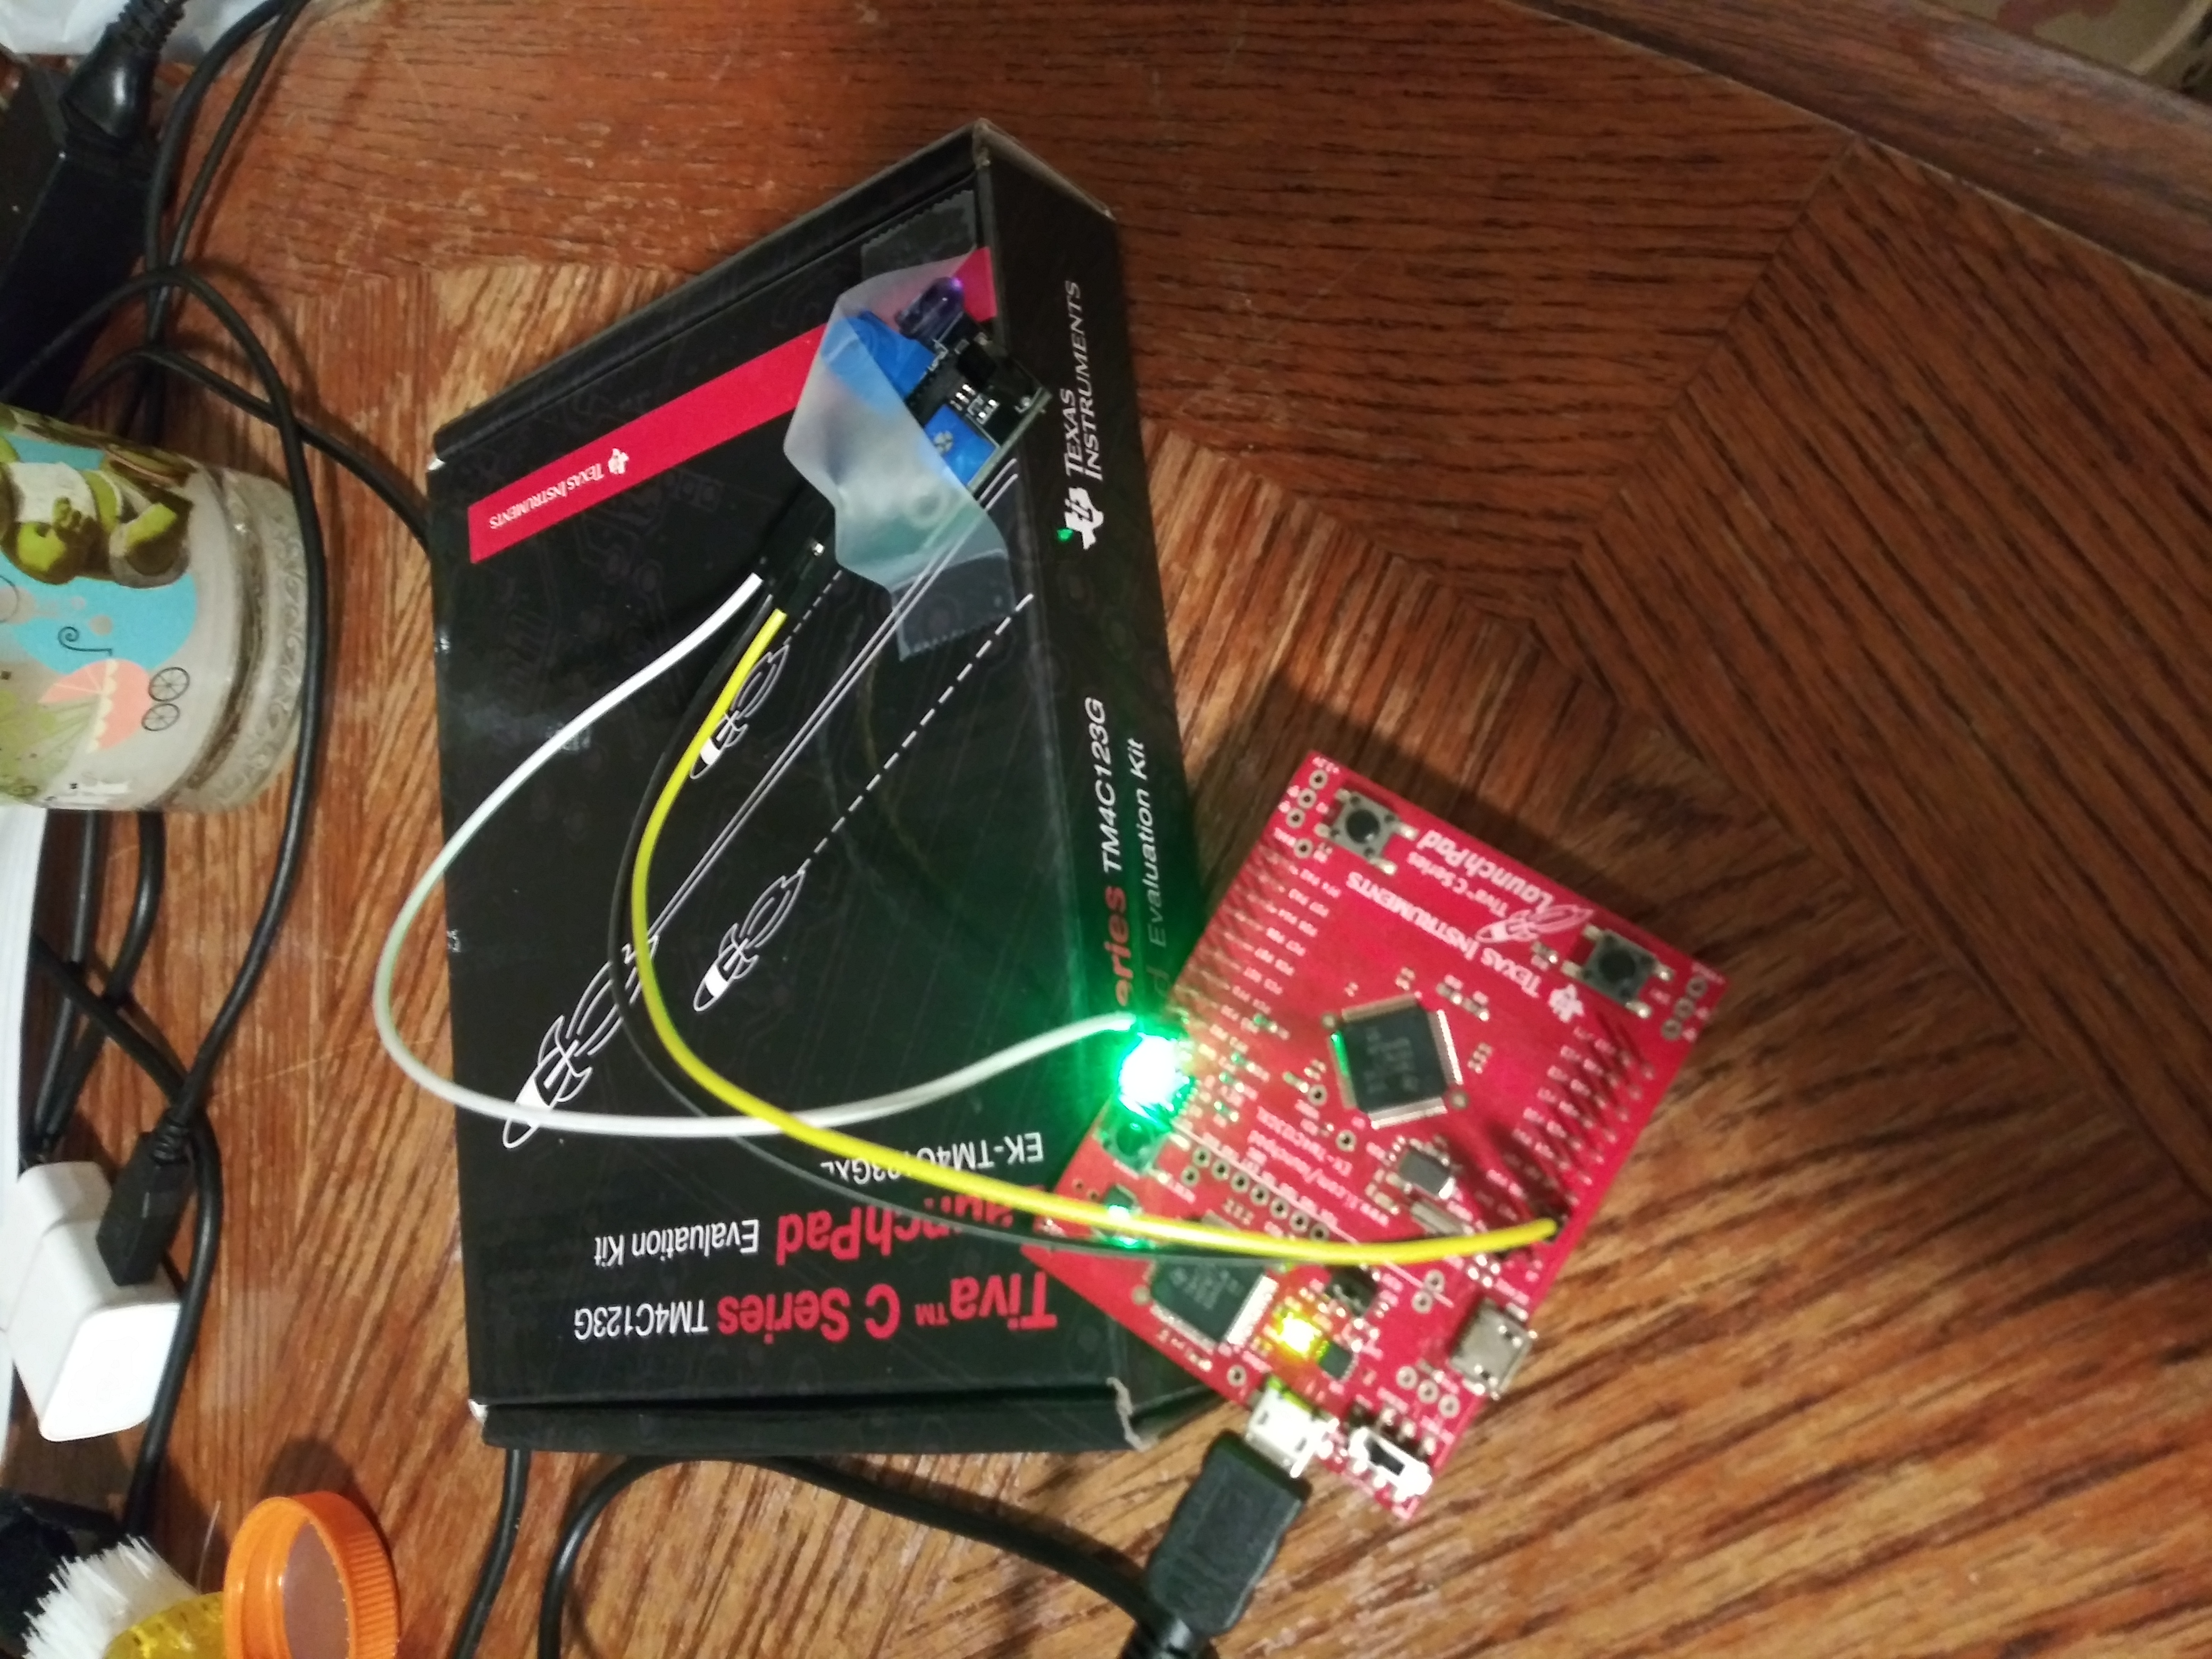
\includegraphics[width=\textwidth, angle=180]{Images/20201202_005731}
    \caption{Image of system running.}
    \label{image}
\end{figure}
\end{itemize}

\end{document}
